\section{Background}
\label{IntroBackground}

Todo,
Future Roland will have to check this content

Swiss Post is Switzerland’s national service provider, active not only in mail and parcel logistics but also in passenger transport (PostAuto), financial services (PostFinance), and various digital and e-government solutions. Its workforce of approximately 45’000 employees and nationwide infrastructure move millions of items and people every day, supported by highly automated sorting centres and extensive data flows \cite{postGeschäftsbericht2024}. In such a diversified organisation, \gls{analyticalreporting} is essential for strategic steering, operational planning, and maintaining service quality across business units. The organisational structure of Swiss Post is shown in the following diagram.

\begin{figure}[H]
    \centering
    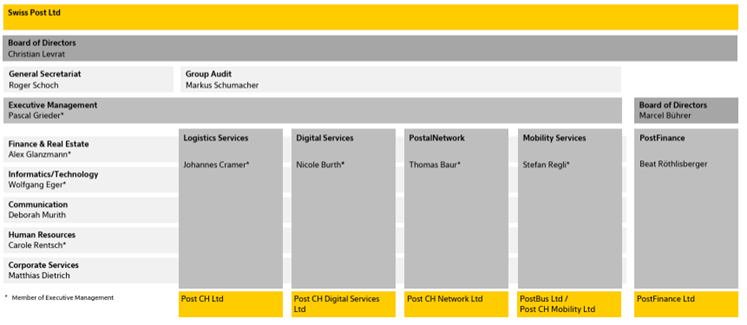
\includegraphics[width=0.8\textwidth]{./content/img/Post_external/OrgStruktur_Online.png}
    \caption{Organisational structure of Swiss Post (online version)}
    \label{fig:orgstruktur_online}
\end{figure}


\subsection*{The full mail piece lifecycle}
Within this large organisation, the project takes place within a specialised team supporting the entire lifecycle of logistics for mail and parcel delivery. In German, this lifecycle covers every step from A to Z, \gls{ASTVZ}, which stands for:
\begin{itemize}
    \item \textbf{A}nnahme: Receiving, where parcels and mail are accepted and registered by Swiss Post to be sent through its network
    \item \textbf{S}ortierung: Sorting, the process during which received mail pieces are separated by destination and routed to the next process step, either further sorting or delivery
    \item \textbf{T}ransport: Transport includes the movement between sorting plants and delivery sectors
    \item \textbf{V}erzollung: Customs clearance handles international parcels and letters, including the required customs checks and documentation
    \item \textbf{Z}ustellung: Delivery is the final process step for every item; it is delivered by the staff of Swiss Post
\end{itemize}

However, this process is more easily visualised using the future vision of Swiss Post. In particular, the version tailored for the IT domain is well suited to describing the project environment. Starting from the top left with the A or V step, followed by S, T, and Z, the process progresses towards the bottom right.

\begin{figure}[H]
    \centering
    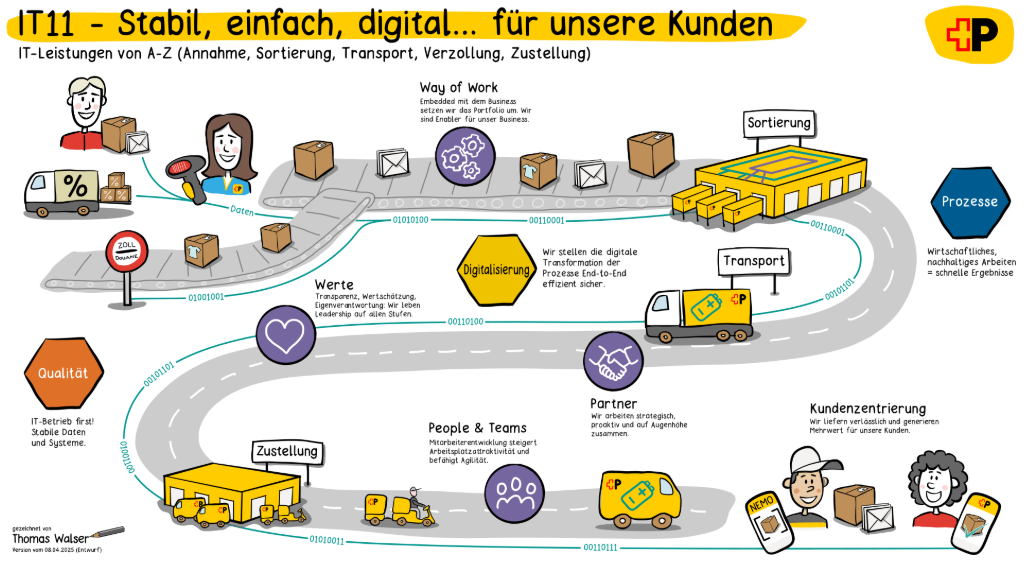
\includegraphics[width=0.8\textwidth]{./content/img/Post_internal/06-12-2025_20-16-16.png}
    \caption{Future way of work illustrating the full postal delivery workflow from receiving an item to delivery.}
    \label{fig:future_way_of_work}
\end{figure}


\subsection*{DWH LS OPS}
\label{IntroDWHLSOPSTasks}

The project team supports the \textbf{D}ata \textbf{W}are\textbf{h}ouse of \textbf{L}ogistic \textbf{S}ervices \textbf{Op}eration\textbf{s} (\gls{DWHLSOPS}). This \textbf{Busi}ness \textbf{Dev}elopment \textbf{Op}eration\textbf{s} (\gls{BizDevOps}) team is located within the organisational structure of the Logistics Services vertical and the Informatics/Technology horizontal. It represents the single source of truth for \gls{analyticalreporting} at Swiss Post. In contrast to operational reporting, which focuses on real-time guidance for operational processes, analytical reporting focuses on aggregated insights for evaluation and planning. Examples of analytical reporting include working time, process time, and aggregations of sorted items. The stakeholders of the team distribute these reports to various task groups within postal services, such as sorting and delivery.

There are two reasons why a deeper understanding of analytical reporting is currently very important. First, the infrastructure for analytical reporting is transitioning from on-premise systems to the cloud. Second, in addition to the migration of reporting, the infrastructure at all Swiss Post \gls{sortingcenter} locations for parcels is undergoing fundamental changes. These changes may include complete modifications of data pipelines, which can make comparisons with previous figures impossible. Therefore, at this critical point in time, it is of utmost importance to maintain users’ trust in the data during this change process. The following figure illustrates the shift from the on-premise setup on the right-hand side to the target architecture using cloud hardware on the left-hand side.

\begin{figure}[H]
    \centering
    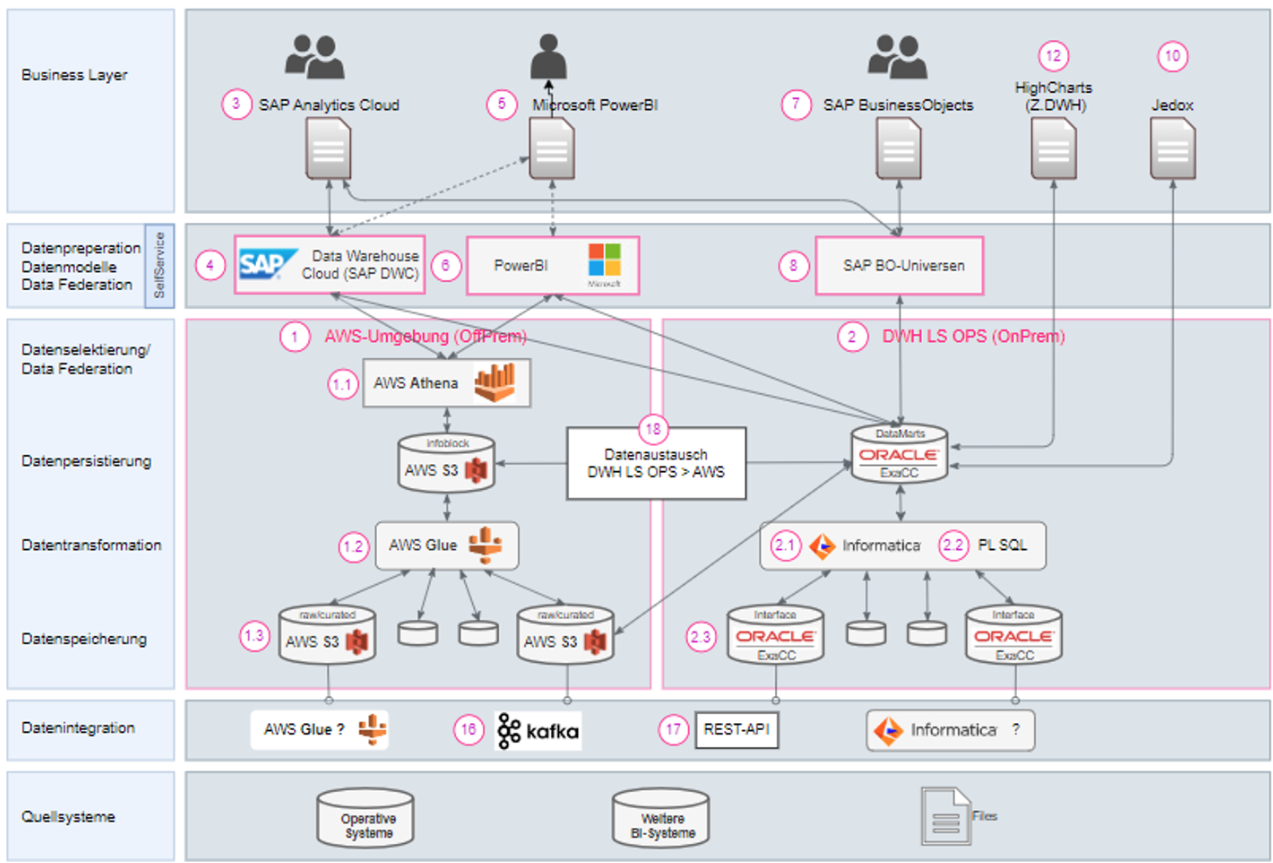
\includegraphics[width=0.8\textwidth]{./content/img/OnPrem_Cloud_Migration.png}
    \caption{The transition from an on-premise setup to a cloud-based target architecture.}
    \label{fig:on_prem_cloud_migration}
\end{figure}


\subsection*{Swiss Post sorting centers are cyber machines}
Swiss Post has built and operate a number of massive sorting centers located across Switzerland. These are far more than just mechanical warehouses or factories. Rather, these sorting centers are massive “cyber facilities” that include high-tech hardware but also high-tech IT systems to keep them running.

While the team handles use cases across the entire postal delivery workflow, this project initially focuses on supporting sorting data flows. Sorting at Swiss Post is the process of consolidating received items in centralised plants, to which letters and parcels are sent from regions across Switzerland. One such plant is located in Härkingen:

\begin{figure}[H]
    \centering
    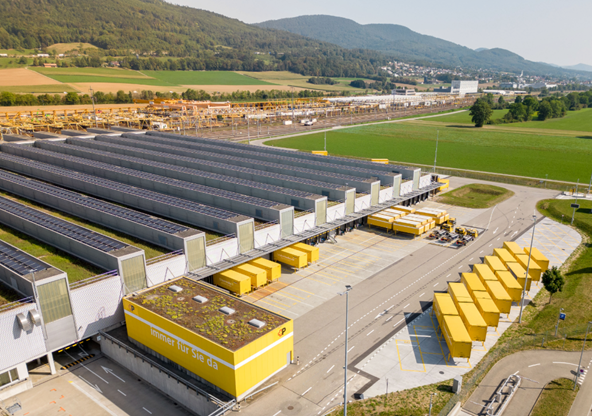
\includegraphics[width=0.8\textwidth]{./content/img/Post_external/Sortierzentrum_Aussen_Vogel.png}
    \caption{Aerial view of the Swiss Post sorting center in Härkingen.}
    \label{fig:sortierzentrum_haerkingen_aerial}
\end{figure}

Mail pieces are handled by workers and placed onto the automated sorting hardware of Swiss Post. This hardware enables the handling of up to 10’000 parcels per hour \cite{SwissPostHarkingenSort}. The system scans the received items and transports them through the plant via conveyor belts to their correct destinations, where they are discharged through chutes. These chutes are shown in the second image, including staff placing the parcels into roll boxes for further processing.

\begin{figure}[H]
    \centering
    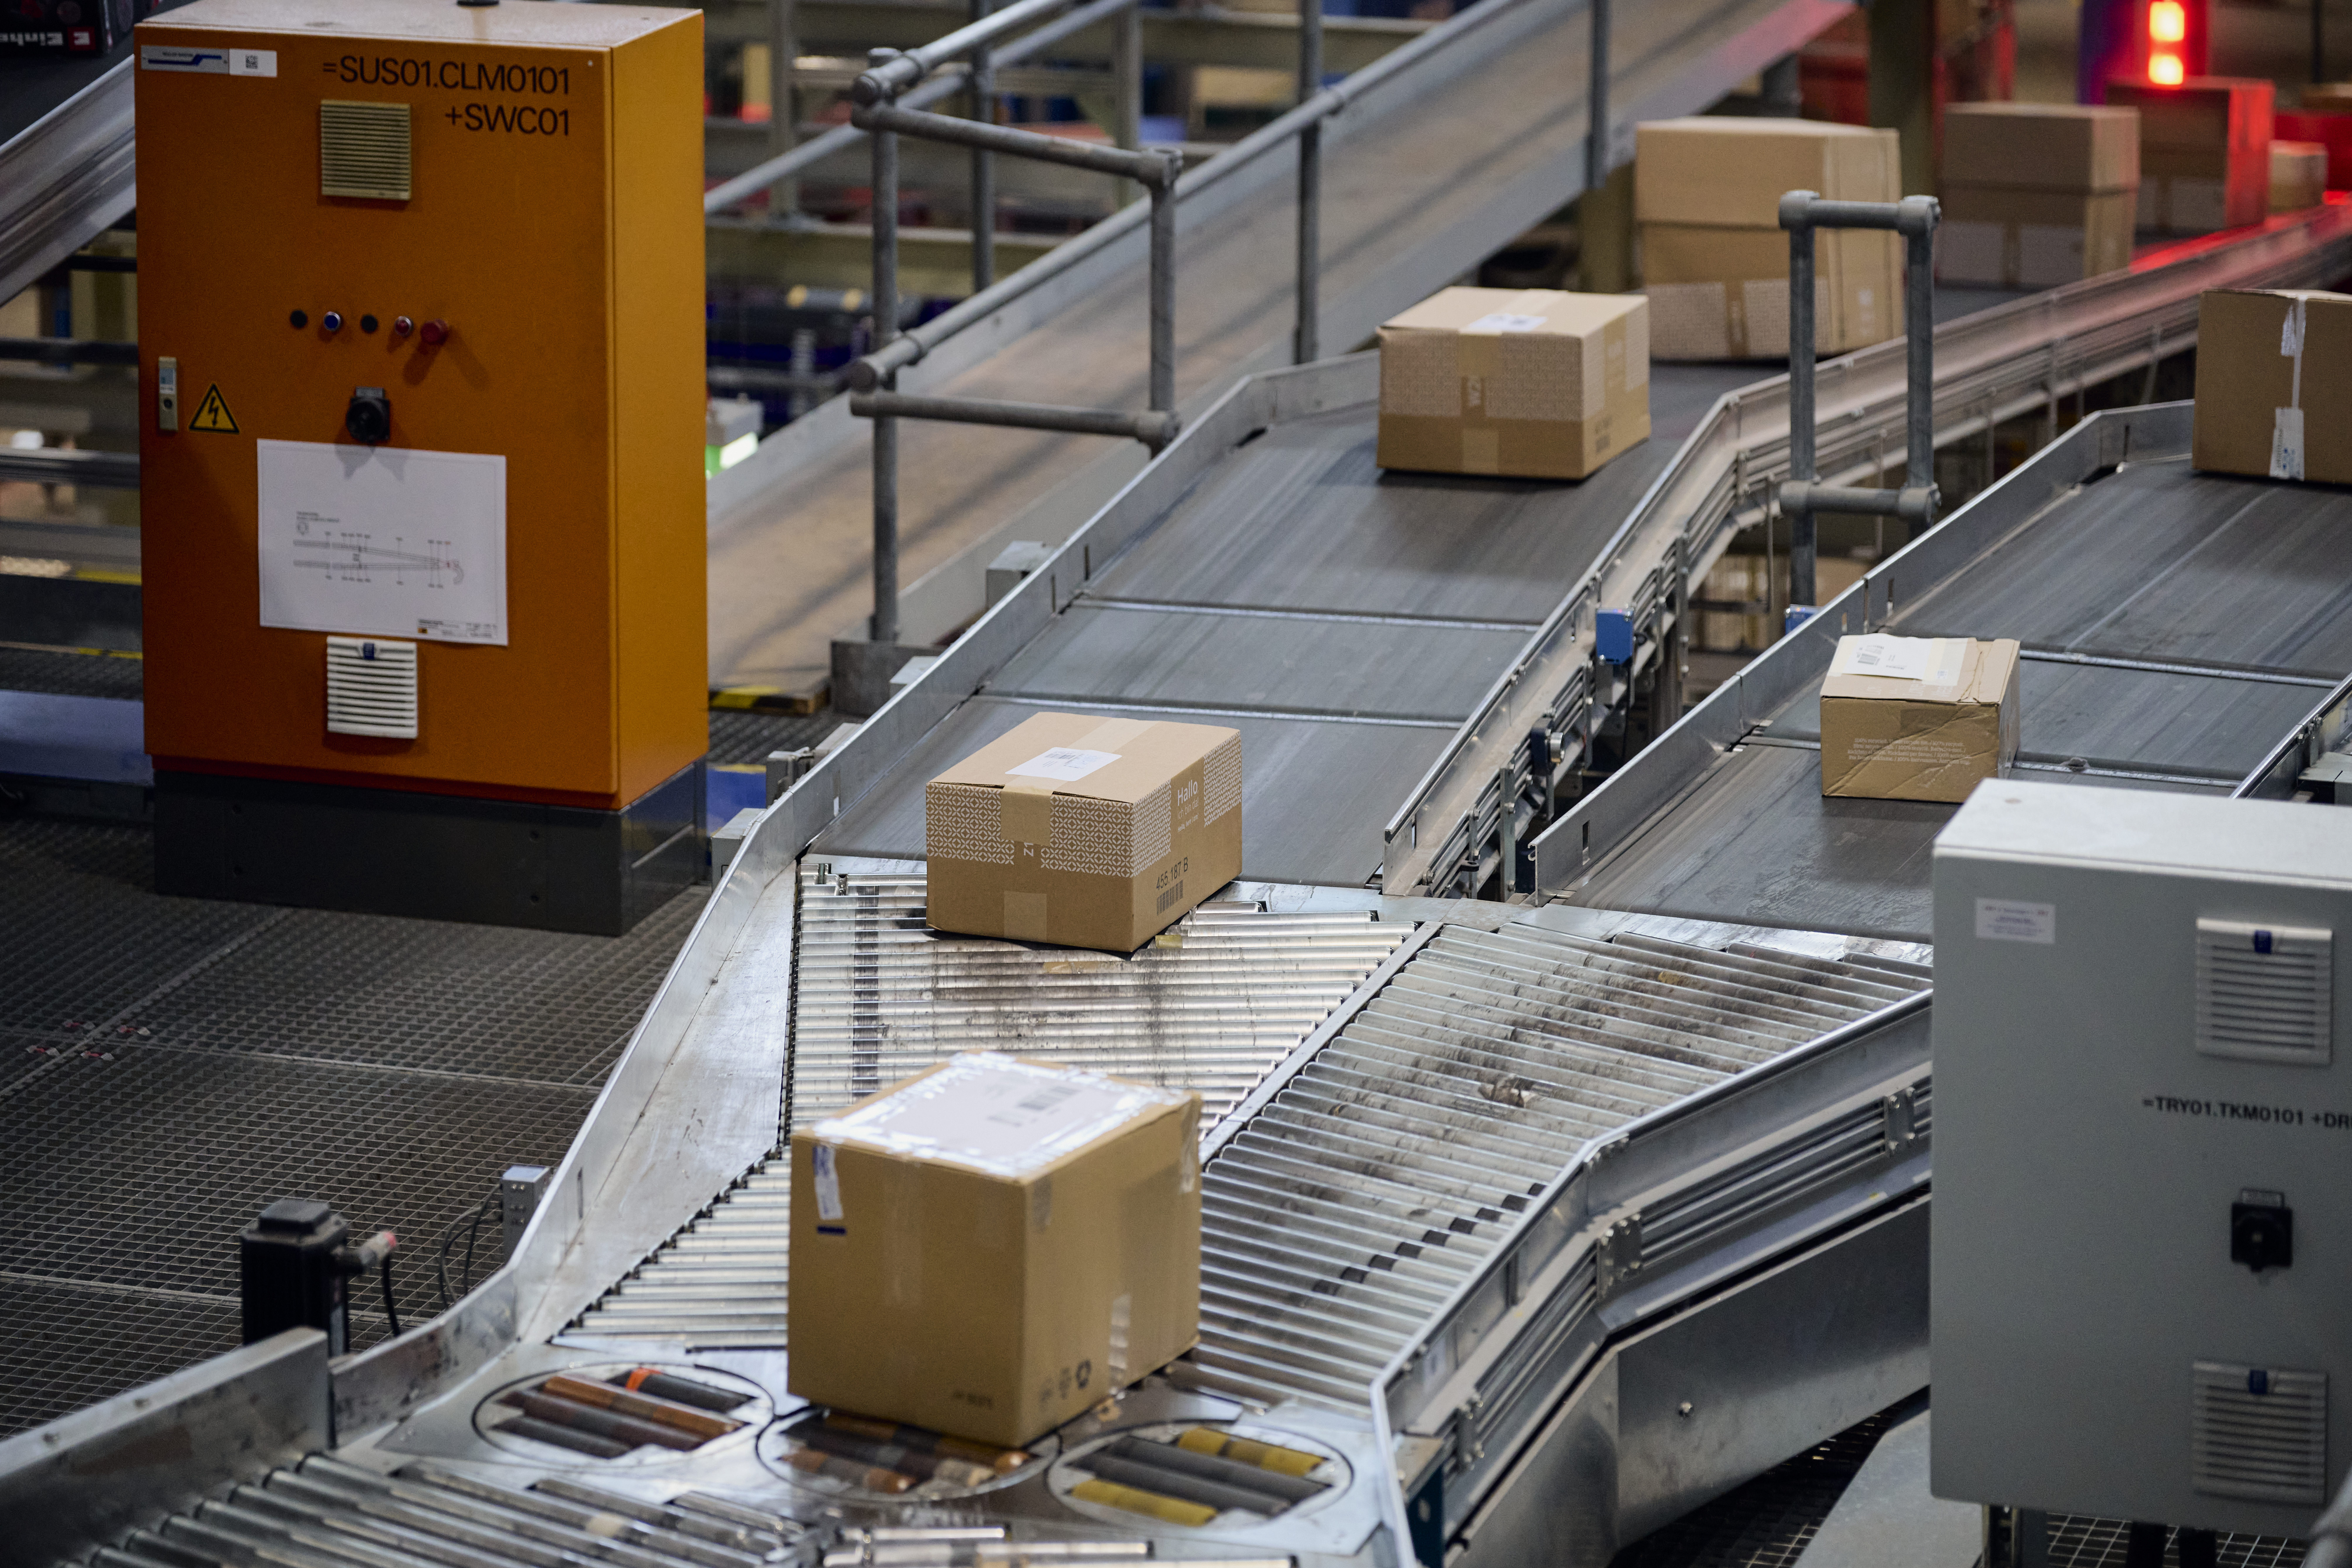
\includegraphics[width=0.8\textwidth]{./content/img/Post_ExperienceHub/_DSC4975.jpg}
    \caption{Interior view of the automated sorting system in a Swiss Post sorting center.}
    \label{fig:sortierzentrum_innen_anlage}
\end{figure}
\begin{figure}[H]
    \centering
    
\includegraphics[width=0.8\textwidth]{./content/img/Post_ExperienceHub/_DSC4916.jpg}
    \caption{Discharge chutes inside a Swiss Post sorting center, where parcels are released to their designated zones. Then put into rollboxes to get them to next processing steps.}
    \label{fig:sortierzentrum_innen_rutschen}
\end{figure}
